% Comment to allow building from within this file
%!TEX root = pyconuk2016.tex

\blankscreen{
}

\begin{frame}{The Logical Paradigm}

    \tikzstyle{hidden} = [
        rectangle, rounded corners,
        % line width=0.4mm, draw=green,
        minimum height=3cm, minimum width=4cm
    ]
    \tikzstyle{individual} = [
        rectangle, rounded corners, line width=0.4mm, draw=blue,
        minimum height=2cm, minimum width=3cm
    ]
    \tikzstyle{class} = [
        ellipse, line width=0.4mm, draw=blue,
        top color=white, bottom color=blue!20,
        minimum height=2cm, minimum width=3cm, align=center
    ]
    \tikzstyle{tuple} = [
        circle, line width=0.4mm, draw=red,
        top color=white, bottom color=red!20,
        minimum height=1cm
    ]
    \tikzstyle{line} = [line width=0.5mm]

    \begin{center}
        \resizebox{10cm}{!}{
            \begin{tikzpicture}

                \node[hidden](0) at (270:5) {};
                \node[hidden](1) at (0:0) {};
                \node[hidden](2) at (0:10) {};
                \node[hidden](3) at (0:5) {};
                \node[hidden](4) at (333:11) {};
                \node[hidden](5) at (346:8) {};

                \node<1-> (photo) at (0){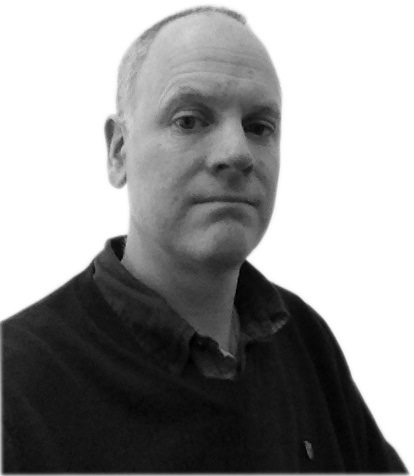
\includegraphics[width=2cm]{images/owencampbell}};

                \node<2-> [individual](owen) at (1) {Me};
                \draw<2-> (photo) -- (owen);

                \node<3-> [class](persons) at (2) {Persons};

                \node<4-> [tuple](t1) at (3) {};
                \draw<4-> (t1) -- (owen) {};
                \draw<4-> (t1) -- (persons) {};

                \node<5-> [class](class-member) at (4) {Class-Member\\ Tuples};

                \node<6-> [tuple](t2) at (5) {};
                \draw<6-> (t2) -- (class-member);
                \draw<6-> (t2) -- (t1);


            \end{tikzpicture}
        }
    \end{center}

\end{frame}
